\chapter{Механизмы памяти в нейросетевых архитектурах}\label{ch:ch1}


\section{Функции, выполняемые памятью}\label{sec:ch1/sec1}

Память выполняет ключевую функцию в процессах когнитивного восприятия, обучения и логического мышления. В рамках обсуждения её можно представить как систему хранения данных с двумя основными функциями: \textit{Запись}, обновляющая данные на основе поступающей извне информации, и \textit{Чтение}, обеспечивающее доступ к сохранённой информации. В машинном обучении память играет важную роль, позволяя системам приобретать и сохранять навыки, которые необходимы для выполнения задач на основе множества обучающих примеров.

Память в машинном обучении используется в различных формах. Некоторые механизмы специально разрабатываются для имитации функций памяти, другие же создаются с иными целями, но могут быть интерпретированы с точки зрения памяти. Главная задача памяти в алгоритмах машинного обучения — сохранять полученные во время обучения шаблоны и навыки. Эту функцию можно сравнить с долгосрочной памятью человека, особенно процедурной или имплицитной памятью, которая поддерживает навыки на протяжении длительного времени.

Связь памяти с понятием времени очевидна. Если задачи обладают временной структурой или требуют обработки последовательных данных, память становится естественным средством связывания временных шагов между собой. Для работы с временными зависимостями применяются механизмы кратковременной памяти, такие как рекуррентные сети или механизмы внимания. Механизмы долговременной памяти чаще всего основываются на явном хранении данных и структурированных операциях. Различные классы таких механизмов и их применение будут рассмотрены далее.

Ещё одна важная область, требующая интенсивного использования памяти, — это задачи, где решение состоит из нескольких последовательных шагов. Примеры включают логическое рассуждение, решение математических задач и другие сложные процессы. В глубоком обучении такие задачи решаются с помощью моделей, где каждый слой выполняет отдельный этап. В этом контексте память используется для хранения промежуточных результатов или других данных, необходимых для выполнения задачи. Этот вид памяти называется \textbf{Рабочей памятью} и отличается тем, что её операции не зависят от внешних данных.

Интересным свойством памяти является её имплицитность или эксплицитность. Некоторые знания, такие как способность ходить или распознавать различия между кошкой и собакой, трудно выразить словами. Имплицитные данные обычно хранятся в сжатом виде, что исключает излишние детали для достижения большей обобщённости, хотя это может сопровождаться потерей части информации. Явные знания, такие как <<кошка — это животное>> или конкретные факты, напротив, хранятся без потерь, но могут включать лишнюю информацию. Явная память не подвергается сжатию и используется только по назначению, в то время как хранилища, выполняющие сжатие или фильтрацию данных, относятся к имплицитным. Аналогично, операции называются явными, если они служат исключительно памяти, и имплицитными — если их функции шире.

Эффективность памяти определяется ёмкостью хранилища и качеством операций чтения и записи. Объём хранилища ограничивает количество информации, а операции должны быть спроектированы так, чтобы использовать его максимально эффективно. Кроме того, они должны поддерживать такие функции, как фильтрация, забывание, выбор данных по содержимому или местоположению, перезапись и другие. Эти аспекты будут подробно рассмотрены в следующих разделах.

Цель данного исследования — классифицировать механизмы нейросетевых архитектур, связанные с использованием хранилища, чтением и записью данных, через призму памяти. Опираясь на свойства таких операций, возможно построить нейронные архитектуры, оптимизированные для задач, требующих интенсивной работы с памятью, с фокусом на обработку естественного языка.


\begin{figure}
    \centering
    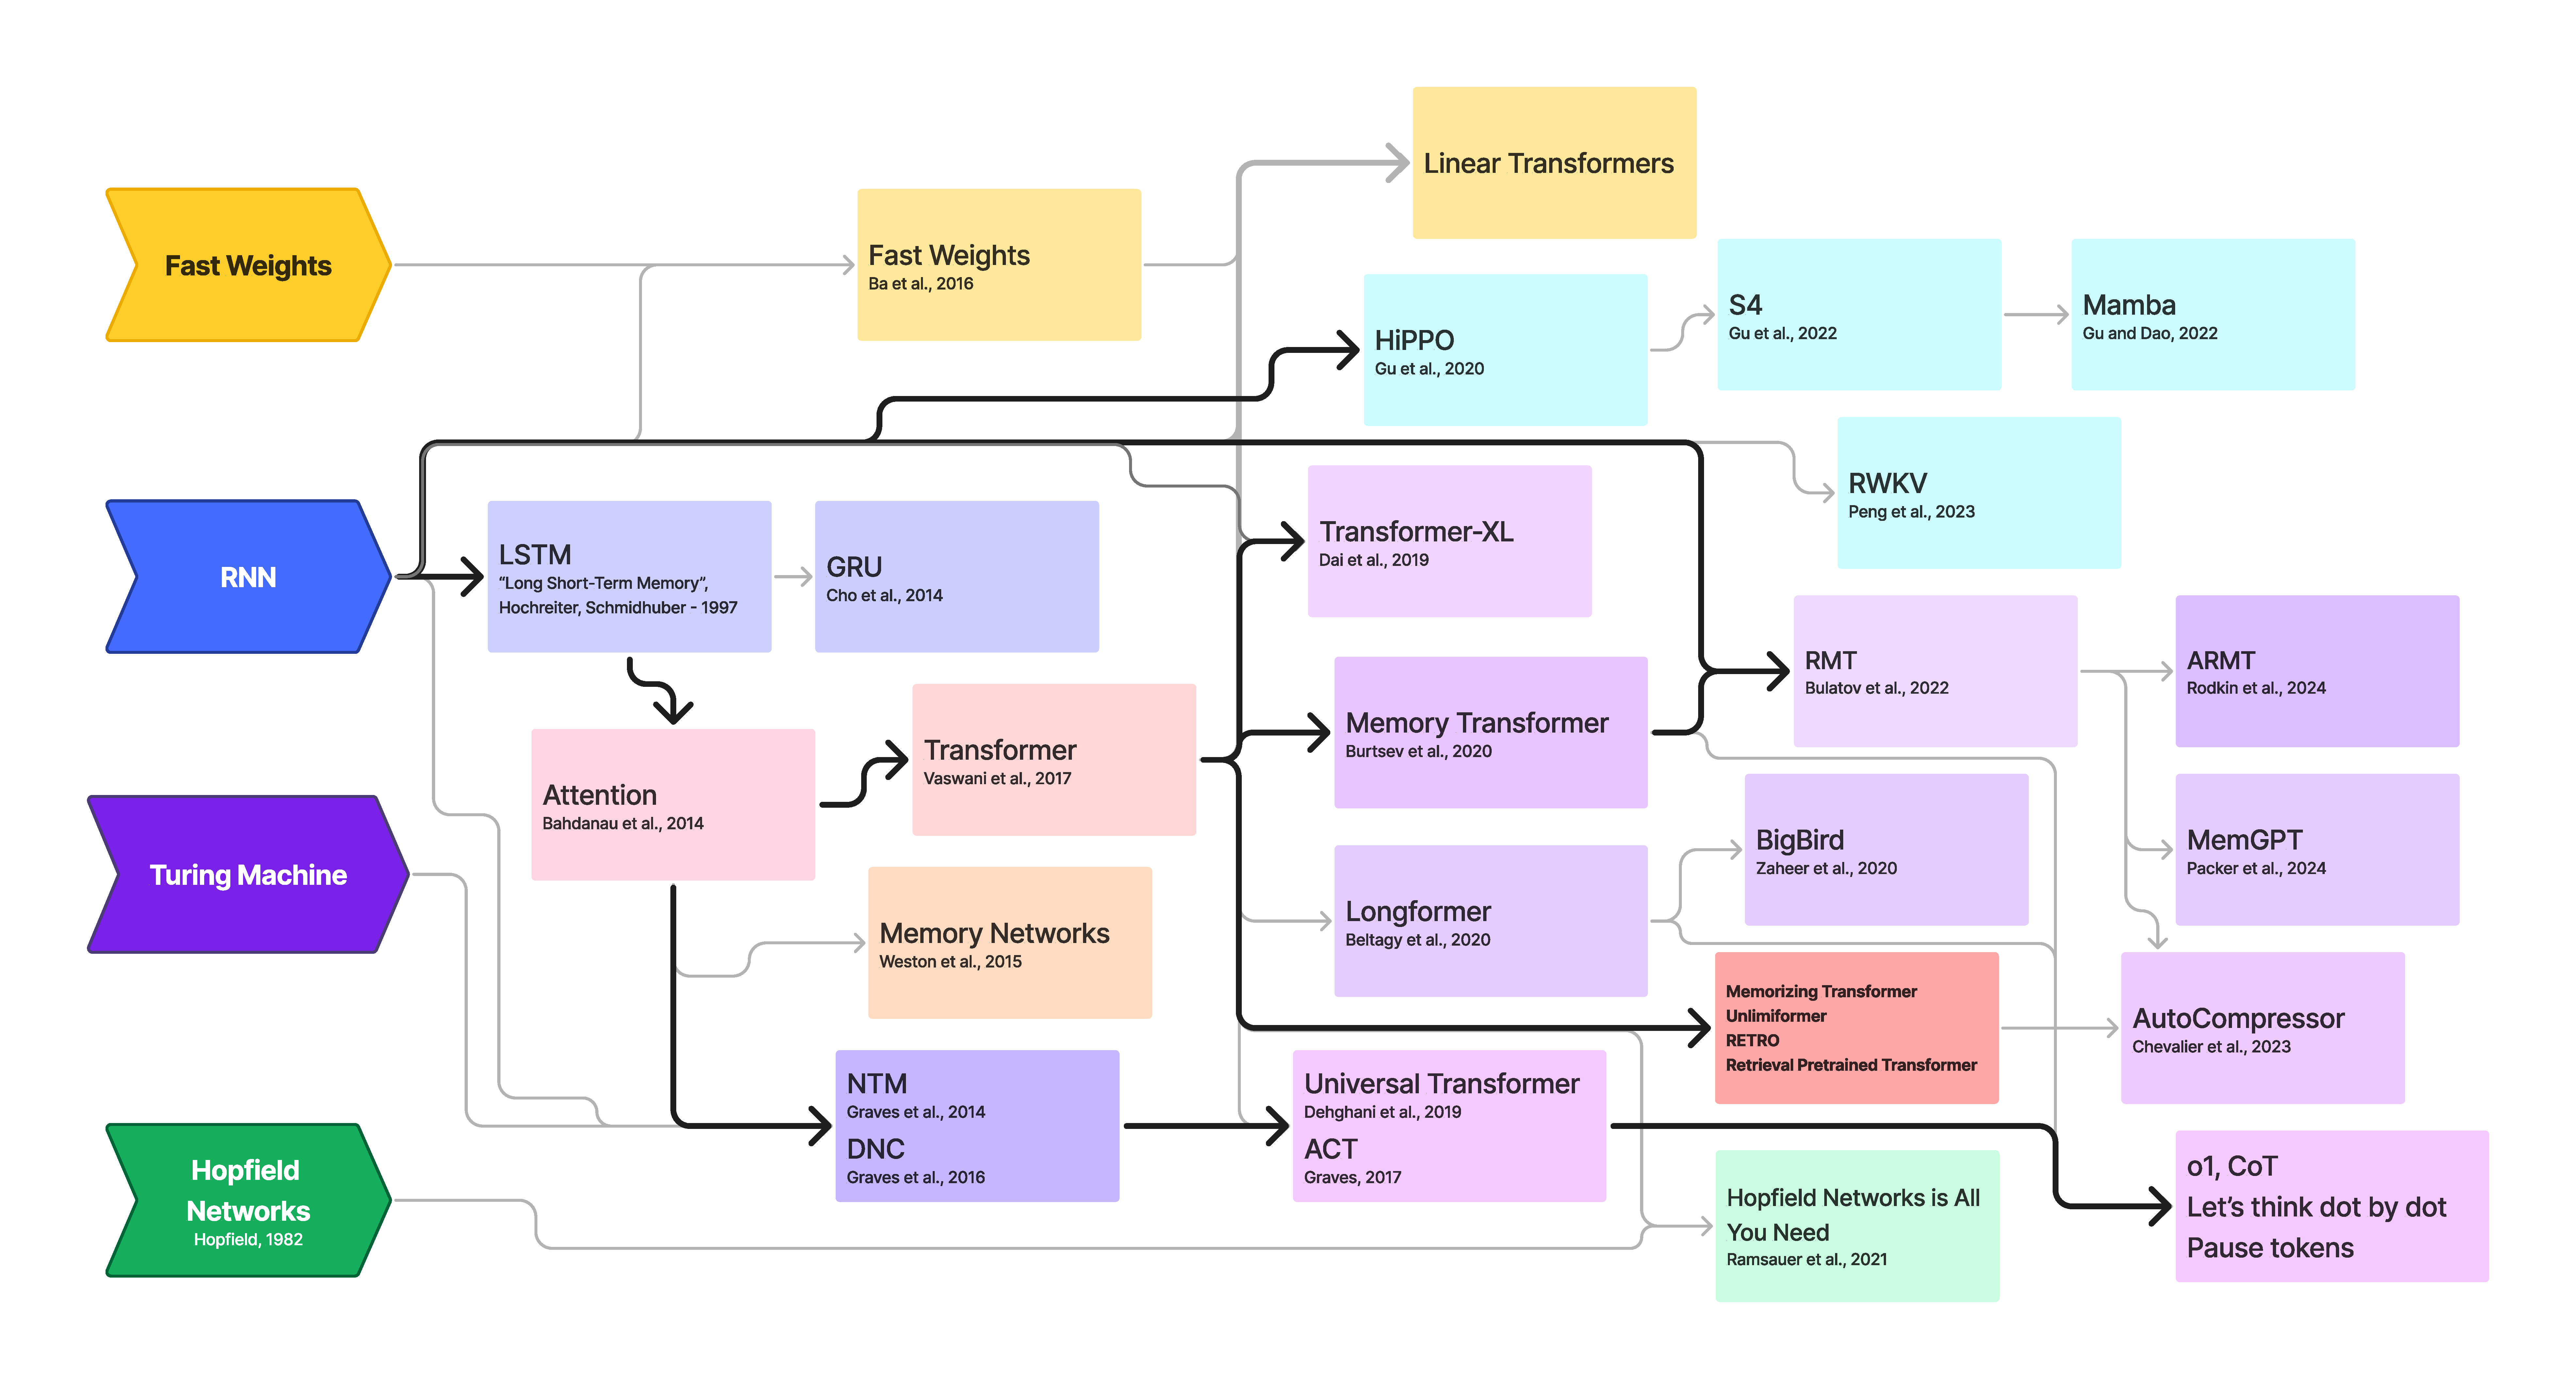
\includegraphics[width=0.95\linewidth]{images/part1/MANN history.pdf}
    \caption{История развития основных нейросетевых архитектур с памятью}
    \label{fig:timeline}
\end{figure}

\section{Ранние подходы к моделированию памяти}
\label{sec:early}

% \todo{Memory in CS vs memory in MANN}
% \todo{Origins of memory types: location-based addressing, content-based addressing==associative memory}

В этом разделе рассматриваются механизмы памяти в машинном обучении и нейронных сетях, выделяя их уникальные особенности по сравнению с традиционными системами памяти, в вычислительных устройствах. В отличие от обычной памяти, где применение операций заранее определено, модели машинного обучения должны обучаться взаимодействию с памятью в процессе тренировки. Это создает дополнительные сложности, связанные с обучением таких операций и их обобщаемостью на другие наборы данных. Таким образом, механизм доступа должен быть способен динамически адаптироваться в зависимости от входных данных модели.

Существуют два основных подхода к организации доступа к памяти: адресация по местоположению и адресация по содержимому. В первом случае местоположение нужной информации известно заранее, и данные извлекаются из конкретного места. Однако этот подход не работает, если структура или содержимое памяти имплицитны, либо не существует отдельных локаций в памяти. В таких ситуациях становится необходимым использование адресации по содержимому.

\subsection{Ассоциативная память}

Одной из ключевых задач ранних исследований в области моделирования памяти было внедрение механизма адресации по содержимому. Этот метод предполагает извлечение информации на основе ее связи с запросом, а не физического местоположения в памяти. Первые модели ассоциативной памяти хранили данные в виде паттернов активации нейронов, как показано в ранних работах~\cite{willshaw1969non}. Позднее эти концепции были улучшены через использование голографической памяти~\cite{plate1995holographic} и высокоуровневых ассоциативных структур~\cite{hinton1981parallel}.

В 1982 году Джон Хопфилд предложил общую модель ассоциативной памяти~\cite{hopfield1982neural}. Его подход основывается на использовании весовой матрицы $W$, которая формируется как сумма внешних произведений NN бинарных паттернов $\{x_i\}_{i=1}^N$, $x_i \in \{-1, 1\}^d$, а $d$ — длина паттерна. Для извлечения ассоциаций из состояния $\xi$, система итеративно обновляет $\xi$, умножая его на $W$, вычитая пороговый вектор $b$ и применяя функцию взятия знако до достижения сходимости:

$$
\textcolor{R}{W = \sum_{i=1}^N x_i x_i^T}, \quad \textcolor{B}{\xi_{t+1} = \text{sgn}(W \xi_t - b)}
$$

Этот процесс имеет теоретические гарантии сходимости к локальному минимуму, поскольку правило обновления минимизирует некоторую энергетическую функцию. Современные исследования стремятся увеличить ёемкость и другие характеристики ассоциативной памяти, предлагая альтернативные энергетические функции~\cite{krotov2016dense, krotov2018dense} и интегрируя эти модели в архитектуры для обработки последовательностей~\cite{danihelka2016associative, ramsauer2020hopfield}.

\subsection{Память в весах модели}

Развитие методов градиентного спуска и обратного распространения ошибки~\cite{ivakhnenko1965cybernetic, werbos1982applications, rumelhart1986learning} позволило обучать сложные универсальные архитектуры для различных задач. В этой парадигме веса ww нейронной сети служат имплицитной памятью, запоминая паттерны из обучающих данных. Эти веса корректируются итеративно через обновления градиента и используются для предсказаний на новых данных:

$$
\textcolor{R}{\theta_{t+1} = \theta_t - \gamma \nabla F (\theta_t)}
$$

$$
\textcolor{B}{\hat{y}_t = f(x_t, \theta_t)}
$$

Здесь $\gamma$ обозначает скорость обучения, а $\nabla F$ — градиент функции потерь. Дополнительные улучшения, такие как стохастический и мини-батч градиентный спуск а также механизмы улучшения сходимости, повысили эффективность обучения моделей~\cite{adam}.

Однако использование только весов в качестве памяти имеет свои ограничения. Градиентные обновления требуют значительного числа итераций и четко определенной функции потерь. Получение новых знаний часто требует дополнительного обучения, которое требует изменения весов модели. Кроме того, обучение на новых данных может приводить к полному стиранию ранее усвоенной информации, известному как \textit{катастрофическое забывание}~\cite{mccloskey1989catastrophic}. Это ограничение обусловлено имплицитным характером памяти в весах.

\subsection{Модели с быстрыми весами}

Для решения проблем медленных обновлений в традиционных весах была предложена концепция \textit{быстрых весов}. Эти веса обновляются чаще традиционных весов и не зависят от явной функции потерь. Ранние работы~\cite{hinton1987using} опирались на исследования~\cite{von1994correlation, feldman1982connectionist}, рассматривая быстрые веса как краткосрочную ассоциативную память для временного обучения и рекурсивной обработки.

Быстрые веса также интегрируются в различные архитектуры нейронных сетей для улучшения свойств запоминания. Например, в~\cite{schmidhuber1992learning} быстрые веса используются как вспомогательный механизм памяти в рекуррентных нейронных сетях (Recurrent Neural Network, RNN). Быстрые веса вычисляются на основе входных данных и выходов RNN на каждом временном шаге и служат адаптивным хранилищем временных переменных:

\begin{align*}
&\textcolor{R}{a_i, b_i = W_a x_i, W_b x_i} \\
&\textcolor{R}{W_i = \sigma(W_{i-1} + a_i \otimes b_i) } \\
&\textcolor{B}{y_i = W_i x_i} \\
\end{align*}


Современные работы, такие как~\cite{ba2016using}, используют аналогии с рабочей памятью для разработки модели быстрых весов, которые динамически восстанавливаются из представлений на текущем временном шаге. Быстрая ассоциативная память двействует в промежутке между временными шагами, постепенно восстанавливая и записывая ассоциации в матрицу быстрых весов. ~\cite{schlag2021fastweights} показывают формальную эквивалентность линейного механизма внимания и контроллера, основанного на быстрых весах. На основе этого наблюдения разрабатывается модель с повышенной ёмкостью памяти. Подробнее эквивалентность разных классов моделей будет рассмотрена в следующих секциях.

\section{Память в архитектурах для обработки последовательностей}
\label{sec:mann}

Некоторые задачи требуют обработки последовательностей, происходящих из различных источников, таких как процессы с временной зависимостью, временные ряды, дискретные и непрерывные сигналы, речь и текст. Для работы с последовательностями переменной длины часто используется рекуррентная обработка, когда элементы обрабатываются по очереди с помощью одинакового набора весов. Это позволяет сохранить фиксированное количество параметров модели, вне зависимости от длины последовательности. Рекуррентный способ обработки последовательных данных предполагает поэтапное выполнение операций: от первого элемента последовательности \( x_1 \) до последнего \( x_L \), где \( L \) — длина последовательности.

\subsection{Рекуррентные нейронные сети}

Рекуррентные нейронные сети (RNN) — это класс нейронных архитектур, специально предназначенных для обработки последовательной информации. Как указано в~\cite{schmidhuber2022annotated}, первые аналоги RNN без обучения появились ещё в 1920-х годах~\cite{lenz1920beitrag}, их обсуждение можно найти в~\cite{mcculloch1943logical}. Впервые обучаемые модели RNN были предложены в~\cite{amari1972characteristics}. Главной особенностью RNN является использование одинаковых весов на всех временных шагах. Это означает, что один и тот же набор весов модели обрабатывает каждый элемент последовательности, получая его на вход вместе с рекуррентным состоянием системы \( s \). Данный процесс описывается системой:

\[
s_t = f(s_{t-1}, x_t, \theta),
\]

где \( f \) — это рекуррентная функция, параметризованная с помощью \( \theta \). Состояние \( s_t \) включает в себя всю информацию о предыдущих шагах, а функция \( f \) выполняет обновление состояния и обработку входных данных.

В данной работе рассматривается упрощённая версия RNN, построенная на базе полносвязных слоёв с весами \( W \), смещениями \( b \), нелинейной функцией активации \( \phi \) и скрытым состоянием в виде вещественного вектора \( h_t \). На каждом шаге времени \( t \) модель принимает \( x_t \) и \( h_{t-1} \) в качестве входных данных и формирует выходной сигнал \( y_t \).

Рекуррентные соединения выполняют роль кратковременной памяти, сохраняя данные о предыдущих шагах. Такие соединения можно сравнить с обратными связями в человеческом мозге, которые позволяют узлам взаимодействовать между собой.

Обучение RNN с использованием метода обратного распространения ошибки во времени (BPTT)~\cite{werbos1988generalization, williams1992gradient} требует прохождения градиента через рекуррентные связи к предыдущим временным шагам. Однако по мере увеличения числа шагов это становится сложнее из-за проблем затухания или взрывного роста градиента, описанных Хохрайтером и Шмидхубером в 1991 году и позже в~\cite{bengio1994learning}. Интуитивно, RNN перезаписывает своё состояние на каждом шаге, что затрудняет сохранение долгосрочной информации. Кроме того, модель не имеет явных механизмов для фильтрации нерелевантных входных данных или удаления устаревшей информации из памяти, возлагая эти задачи на основной слой.

\subsection{Сети долгой краткосрочной памяти}

Архитектура с длинной краткосрочной памятью (Long Short-Term Memory, LSTM)~\cite{lstm1999hochreiter} представляет собой усовершенствованную версию RNN, добавляющую отдельное состояние памяти, которое хранится и обрабатывается независимо. Этот подход создаёт дополнительное пространство для хранения информации, что позволяет сохранять больше данных на длительных интервалах времени. Работа с памятью в LSTM осуществляется с помощью отдельных элементов управления: гейта забывания (\( f \)), входного гейта (\( \mathbf{i} \)), гейта, генерирующего кандидатное состояние ячейки (\( \tilde{c} \)), и выходного гейта (\( o \)).


\begin{align*}
    &\textcolor{R}{h_t = f_t \odot h_{t-1} + i_t \odot \tilde{h_t}}, \quad \text{where} \\
    &\textcolor{R}{f_t = \sigma (x_t W_{xf} + o_{t-1} W_{hf} + b_f)} \\
    &\textcolor{R}{i_t = \sigma (x_t W_{xi} + o_{t-1} W_{oi} + b_i)} \\
    &\textcolor{R}{\tilde{h}_t = \tanh (x_t W_{xh} + o_{t-1} W_{oh} + b_h)} \\[1ex]
    &\textcolor{B}{o_t = \tilde{o}_t \odot \tanh (h_t)}, \quad \text{where} \\
    &\textcolor{B}{\tilde{o}_t = \sigma (x_t W_{xo} + o_{t-1} W_{oo} + b_o)}
\end{align*}

Для выполнения операций используются произведение Адамара (\( \odot \)), а также функции активации, такие как сигмоида (\( \sigma \)) и гиперболический тангенс (\( \tanh \)). В данной статье переменные переименованы для единообразия терминологии: \( h_t \) обозначает состояние памяти, а \( o_t \) — выход ячейки, также передаваемый на следующий шаг.

Раздельное хранение и обработка памяти позволяет в LSTM добиться «постоянного потока ошибки» на этапе обратного распространения, что даёт возможность эффективно обучать модель на задачах с долгосрочными зависимостями. Благодаря этому LSTM приобрела популярность как в академических исследованиях, так и в промышленности, решая задачи от автозаполнения текста до обработки сигналов и машинного перевода.

Gated Recurrent Unit (GRU)~\cite{cho2014gru}, являющийся упрощённой версией LSTM, уменьшает сложность архитектуры за счёт объединения гейта забывания и гейта обновления в единый механизм. GRU использует одно состояние памяти, что упрощает обучение, при этом обеспечивая результаты, сравнимые с LSTM. Рекуррентные сети также применяются в составе более сложных моделей, таких как двунаправленные RNN~\cite{schuster1997bidirectional} или многослойные нейронные сети~\cite{Peters2018DeepCW}, которые создают более контекстуализированные двунаправленные текстовые представления. Например, метод~\cite{memupsorokin2022} расширяет возможности RNN с помощью внешней памяти и подходов к обучению, нацеленных на элементы последовательности, предсказываемые с высокой степенью неопределённости.

\subsection{Архитектуры с механизмом внимания}

На протяжении длительного времени рекуррентные модели выступали основным инструментом для обработки последовательных данных, включая такие задачи, как преобразование последовательность-в-последовательность и машинный перевод. Однако с увеличением длины последовательностей, подлежащих переводу, рекуррентные модели испытывают сложности с сохранением всей последовательности в скрытом состоянии. Это явление, известное как «узкое место скрытого состояния», обусловлено использованием RNN единственного (ограниченного) состояния памяти фиксированной длины. Для преодоления этой проблемы необходимо обеспечить возможность одновременного доступа к нескольким состояниям памяти.

Предложенная в работе ~\cite{bahdanau2015neural} архитектура кодировщик-декодировщик решает эту задачу. Она сочетает двунаправленную RNN (Bi-RNN) в роли кодировщика и стандартную RNN в роли декодировщика. Ключевым элементом этой архитектуры является «модель выравнивания», встроенная в декодировщик, которая позволяет на каждом этапе генерации учитывать все входные элементы.

Кодировщик
\begin{align*}
&\textcolor{R}{\overleftarrow{h}_{\tau} = \phi(x_{\tau} W_{xh}^b + \overleftarrow{h}_{\tau-1} W_{hh}^b + b_h^b)} \\
&\textcolor{R}{\overrightarrow{h}_{\tau} = \phi(x_{\tau} W_{xh}^f + \overleftarrow{h}_{\tau-1} W_{hh}^f + b_h^f)} \\
&\textcolor{R}{h_{\tau} = [\overrightarrow{h}_{\tau}^T, \overleftarrow{h}_{\tau}^T]} \\[1ex]
\end{align*}

Декодировщик
\begin{align*}
&\textcolor{B}{c_{t} = \sum_{\tau=1}^T \alpha (s_{t-1}, h_{\tau}) h_{\tau}} & \text{} \\
&\textcolor{R}{s_{t} = f(s_{t-1}, y_{t-1}, c_{t})} & \text{} \\
&\textcolor{B}{y_{t} = Y(s_{t})} & \text{}
\end{align*}


Кодировщик Bi-RNN обрабатывает каждое входное слово \(x_{\tau}\), находящееся в позиции \(\tau\), и формирует векторную \textit{аннотацию} \(h_{\tau}\). Эти векторы составляют память кодировщика. На этапе декодирования \(t\) формируется контекстный вектор \(c_t\), который представляет собой взвешенную сумму аннотационных векторов \(h_{\tau}\). Веса, задаваемые моделью выравнивания \(\alpha\), отражают степень релевантности каждого аннотационного вектора \(h_{\tau}\) текущему состоянию памяти декодировщика \(s\). Выходное значение декодировщика \(y_t\) вычисляется путем применения проекции \(Y\) к состоянию памяти декодировщика \(s_t\).

Механизм внимания позволяет устранить проблему узкого места в ограниченном скрытом состоянии, поскольку вместо сжатия в одно состояние, информация распределяется между скрытыми состояниями всех входных элементов. Механизм внимания выступает в роли ассоциативной памяти, которая извлекает данные из нескольких релевантных состояний. Это можно противопоставить традиционным RNN, где вся информация должна быть компактно закодирована в едином состоянии, что требует сложных методов сжатия. Механизмы внимания, напротив, используют распределенное хранилище в роли памяти, а хранимые представления могут быть более простыми и независимыми друг от друга, объединяясь только через внешние операции. Преимущества и недостатки рекуррентных и параллельных механизмов памяти подробно обсуждаются в разделе~\ref{sec:differences}.

Идея внимания получила широкое распространение в исследованиях обработки естественного языка. Она используется совместно с рекуррентностью в таких архитектурах, как Neural Turing Machine (NTM)~\cite{graves2014neural}. Эта модель обладает вычислительными возможностями машины Тьюринга, однако все операции в ней заменены на дифференцируемые, что позволяет обучать её с использованием градиентного спуска. Память NTM разделена на несколько локаций, и каждая операция чтения возвращает взвешенную сумму векторов памяти, что реализует доступ на основе содержимого. Значения внимания вычисляются с использованием косинусного сходства между векторами памяти и ключевым вектором. Также реализован доступ на основе позиции через ротационные сдвиги, что улучшает работу с памятью. Операции записи в память включают этапы «стирания» и «добавления», что обеспечивает сопсобность к фильтрации и удалению информации.

\begin{align*}
&\textcolor{R}{\tilde{M}_t[i] = M_{t-1}[i][1 - w_t(i) e_t]} \text{ - erase} \\
&\textcolor{R}{M_t[i] = \tilde{M}_t[i] + w_t[i] a_t } \text{ - add} \\[1ex]
&\textcolor{B}{r_t = \sum_{i=1}^m w_t[i] M_t[i]} \\
& w_t^c[i] = \text{Softmax}(\beta_t \frac{k_t  \cdot M_t[i]}{||k_t|| \cdot ||M_t[i]||}) \\
& w_t^g = g_t w_t^c + (1-g_t) w_{t-1} \text{ - interpolation}\\
& \tilde{w}_t[i] = \sum_{j=0}^{N-1} w_t^g[j] s_t(i-j)\\
&w_t[i] = \frac{\tilde{w}_t[i]^{\gamma_t}}{\sum_j \tilde{w}_t[i]^{\gamma_t}}
\end{align*}

Каждая голова модели формирует вектор ключей $k_t$ длиной $M$ и скалярный параметр интерполяции $g_t$, принимающий значения в пределах (0,1). Положительный параметр $\beta_t$, называемый силой ключа, регулирует механизм фокусировки, отвечающий за работу внимания.

Нейронные Тьюринговы машины (NTM) стали основой для таких моделей, как \textit{Дифференцируемый нейронный компьютер} (DNC)~\cite{graves2016hybrid} и \textit{Sparse DNC}~\cite{rae2016scaling}. Эти архитектуры представляют собой рекуррентные нейронные сети, которые могут динамически взаимодействовать с памятью в процессе работы. Их дифференцируемая структура позволяет обучать их с использованием метода обратного распространения ошибки через время (Backpropagation Through Time BPTT). В параллельных исследованиях изучаются расширения рекуррентных сетей, таких как LSTM, за счет добавления структур данных, включая стеки, списки или очереди~\cite{arm2015inferring,grefenstette2015learning}.

Описанные выше модели в основном используют память для обработки краткосрочных зависимостей, что напоминает кратковременную память человека. В то же время существуют исследования, направленные на реализацию аналогов долговременной памяти с использованием схожих механизмов. Например, Memory Networks~\cite{weston2014memory} обеспечивают более долгосрочное хранилище с несколькими ячейками памяти и явными операциями над ними. Эти модели включают такие компоненты, как \textit{входная компонента} $I$, \textit{компонента обобщения} $G$, \textit{выходная компонента} $O$ и \textit{компонента отклика} $R$.

\begin{align*}
&\textcolor{R}{x_t \rightarrow I(x_t)} \\
&\textcolor{R}{m_t[i] = G(m_{t-1}[i], I(x_t), m_{t-1})} \\[1ex] %\quad \forall i \in {1, 2, ... m?} \\[1ex]
&\textcolor{B}{o_t = O(I(x_t), m_t)} \\
&\textcolor{B}{r_t = R(o_t)} \\
& O(x, m) = \text{argmax}_i s_o(x, m[i]) / s_o([x, m_{o1}], m[i])\\
& s(x, y) = \Phi_x(x)^T U^T U \Phi_y(y) \\
& r = \text{argmax}_{w \in W}s_r([x, m_{o1}, m_{o2}], w)
\end{align*}



Предложенная архитектура Memory Networks использует функцию внимания для чтения из представления памяти с предыдущих временных шагов и последующей записи, а рекуррентная нейронная сеть отвечает за генерацию последовательностей. Такое разделение задач для разных весов позволяет памяти сосредоточиться на обработке долгосрочных зависимостей. Для решения масштабных задач объем памяти может достигать 14 миллионов состояний. Изначально такие сети требовали специализированных функций потерь для каждой компоненты при оубчении. Однако в последующих исследованиях эта проблема была решена~\cite{sukhbaatar2015endtoend}.

Механизм внимания представляет собой эффективное решение проблемы ограничения объема скрытых состояний, что позволило ему стать стандартом для реализации памяти для обработки последовательностей. С точки зрения памяти внимание снижает необходимость сжимать информацию в одно состояние, позволяя обращаться ко всем предыдущим состояниям сразу. Это увеличивает масштабируемость и ёмкость памяти, но делает операции чтения более ресурсозатратными, так как объем памяти увеличивается с каждым временным шагом.

\subsection{Память в архитектуре Трансформер}

С появлением архитектуры Трансформер~\cite{vaswani2017attention} внимание стало основой стандартных подходов к решению задач на последовательностях. В этой архитектуре рекуррентные структуры были заменены блоками внимания как в кодировщике, так и в декодировщике.

Каждый блок внимания в кодировщике начинается с многоголового внимания, которое выполняет масштабированное скалярное произведение в нескольких параллельных головах, после чего применяютя полносвязные слои. Использование обходных соединений (skip connections) облегчает прямую передачу информации и стабилизирует процесс обучения. В блоках декодировщика дополнительно реализуется механизм перекрестного внимания, который интегрирует контекстные представления из кодировщика, обогащая представления в декодировщике. Также в декодировщике используется каузальная маска внимания, предотвращающая доступ текущего токена к последующим, оставляя доступ только к предыдущим моментам времени.

Для наглядности рассмотрим процесс на уровне одного слоя (хотя Трансформер состоит из нескольких слоев, каждый из которых имеет свою память и уникальные параметры). В задачах преобразования последовательностей скрытые состояния кодера $H_T^e$ можно трактовать как память. Она состоит из представлений $h_{\tau}^e$ для входных токенов $x_{\tau}$, где $\tau = [1, 2, ... T]$, а $T$ — общее число токенов. На временном шаге $t$ декодировщик сохраняет собственную память в виде скрытых состояний $[s_1^d, s_2^d, ..., s_{t-1}^d]$, которые были сформированы на предыдущих шагах.

В кодировщике и декодировщике механизмы внимания записывают информацию в контекстно-зависимые представления ($h_{\tau}^e$ для кодировщика и $c_t^d$ для декодировщика), объединяя данные из различных состояний. Этот процесс можно рассматривать как операцию записи в память. Между тем перекрестное внимание выполняет чтение из этих контекстных представлений, объединяя их для выполнения задачи.


Кодировщик
\begin{align*}
&\textcolor{R}{h_{\tau}^e = \tilde{\text{MHA}}_{\text{self}}^e(x_{\tau}^e, X_{T}^e) } \\
&\textcolor{R}{H_{T}^e = [h_1^e, h_2^e, ..., h_{T}^e]} \\[1ex]
% &\textcolor{R}{} \\[1ex]
\end{align*}

Декодировщик
\begin{align*}
&\textcolor{B}{c_t^d = \text{MHA}_{\text{self}}^d(h_t^d, H_{t0}^d)} \\
&\textcolor{B}{H_t^d = [h_1^d, h_2^d, ..., h_t^d]} \\
&\textcolor{R}{s_t = \tilde{\text{MHA}}_{\text{cross}}^d(c_t^d, H_T^e) } \\
&\textcolor{B}{y_t = \tilde{\text{FF}}(s_{\tau})} \\
\end{align*} 

\begin{align*}
& \tilde{\text{MHA}} (h_t, H_t) = \text{LN}(h_t + \text{MHA} (h_t, H_t)) \\
& \text{MHA} (h_t, H_t) = [\text{head}_1, ..., \text{head}_h] W^o  \\
& \text{head}_i(h_t, H_t)= \text{Softmax}(\frac{q_t K^T}{\sqrt{d}}) V =\\
& =\text{Softmax}(\frac{h_t W_q (H_t W_k)^T}{\sqrt{d}}) H_t W_v \\
& \tilde{\text{FF}} (s) = \text{LN}(s + \text{FF} (s)) \\
& \text{FF}(s) = \phi(\phi(s W_2 + b_2) W_1 + b_1)
\end{align*}


\subsection{Альтернативный взгляд на память в Трансформере}

\begin{figure}
    \centering
    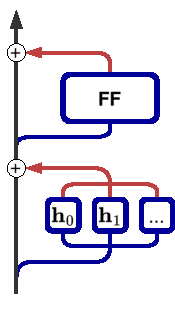
\includegraphics[width=0.4\linewidth]{images/part1/scheme-mechanistic.pdf}
    \caption{Работа с памятью в слоях Трансформера. Головы внимания ($\mathbf{h_i}$) и полносвязный слой ($\mathbf{FF}$) получают данные из общего хранилища, называемого информационным потоком. После выполнения вычислений результаты записываются обратно в этот поток с использованием механизма сложения и нормализации (add-norm), обозначенного плюсом.}
    \label{fig:scheme-mechanistic}
\end{figure}

Операционный подход к работе с памятью, основанный на исследованиях механистической интерпретации~\cite{elhage2021mathematical} в слоях Трансформера представлен на рисунке~\ref{fig:scheme-mechanistic}.

На первом этапе токены проецируются в пространство скрытых представлений, которое служит основным рабочим пространством для обработки данных на каждом слое модели. Обходные соединения, формируют «информационное русло», идущее в обход всех слоев модели. Можно провести аналогию с состоянием ячейки LSTM~\cite{lstm1999hochreiter} или архитектуре Highway Networks~\cite{srivastava2015highway}. Механизмы многоголового внимания (MHA) и полносвязные слои оперируют с определёнными подпространствами этого потока. Их результаты добавляются к текущему представлению и нормализуются, чаще всего с использованием нормировки по слою (LN):  


\begin{align*}
\textcolor{R}{}
& \textcolor{B}{\hat{h}_t = \text{FF} (c_t)}  \quad & \textcolor{R}{h_t = LN(h_t + \hat{h}_t)}\\
& \textcolor{B}{\hat{c}_t = \text{MHA} (x_t, X_T)} \quad & \textcolor{R}{c_t = LN(c_t + \hat{c}_t)}\\
% & X_T = [x_1, x_2, ..., x_T]
\end{align*}

Каждый блок внимания независимо читает и записывает данные в информационный поток. Однако такая структура имеет важное ограничение. Операция внимания объединяет информацию из соседних токенов для создания контекстного представления. При этом это же представление используется в следующих слоях как для извлечения контекста, так и для выполнения задач, что приводит к смешиванию локальных и глобальных признаков в одних и тех же векторах. Такое «размывание признаков» уменьшает эффективность хранения информации в скрытых состояниях. Архитектуры с явной памятью решают эту проблему за счёт выделения промежуточных представлений, таких как шаги рассуждений или вычислений, в отдельное хранилище~\cite{burtsev2020memory-transformer, beltagy2020longformer}. Эти подходы подробно описаны далее.  

В отличие от RNN, Трансформеры в общем случае не обладают встроенной способностью учитывать временные зависимости, поэтому временная информация добавляется с помощью внешних механизмов. Ещё одним ограничением является фиксированная глубина представлений, определяемая числом слоев в Трансформере. В RNN скрытые состояния обновляются на каждом временном шаге, что позволяет увеличивать глубину и степень компрессии хранимой информации. Фиксированная глубина ограничивает выразительные возможности Трансформера и снижает его эффективность в задачах, требующих последовательных рассуждений. Архитектуры, такие как Feedback Transformer~\cite{fan2020feedback-transformer} и Funnel Transformer~\cite{dai2020funnel}, решают эту проблему, вводя связи между слоями для разнообразия путей представления. Universal Transformer~\cite{dehghani2018universal-transformer} добавляет адаптивную рекурсию, применяя тот же слой несколько раз, что увеличивает выразительность модели, аналогично подходам RNN~\cite{graves2016adaptive}. Это позволяет хранить промежуточные результаты между шагами вычислений, повышая способность модели к многошаговому выполнению задач.  

Многие современные исследования сосредоточены на добавлении дополнительных вычислений для улучшения рассуждений. Например, модели могут генерировать дополнительные токены, имитирующие процесс размышления~\cite{wei2022chain}, или вводить специальные токены для повышения способности к рассуждению~\cite{goyal2023think, pfau2024let}. Эти подходы увеличивают выразительность модели за счёт выделения дополнительных ресурсов для выполнения задач.  

\subsection{Неявная память в полносвязных слоях}

Полносвязные слои Трансформера играют важную роль как неявное хранилище памяти. Исследование~\cite{sukhbaatar2019augmenting} предлагает теоретическую переформулировку полносвязных слоев в слое Трансформера, формально эквивалентную механизму внимания с определенным входом. Эти идеи привели к созданию единой архитектуры, где полносвязные слои заменены на механизмы внимания с использованием постоянных векторов, не зависящих от входных данных. Такие модели демонстрируют результаты, сопоставимую с оригинальным Трансформером.  

В других работах~\cite{geva2020transformer} показано, что полносвязные слои эмулируют память в виде пар ключ-значение, где отдельные головы кодируют закономерности, которые доступны к интерпретации. Эти закономерности агрегируются во время выполнения задач, влияя на предсказания модели. Подходы к модификации памяти, такие как редактирование знаний~\cite{meng2022locating, meng2022mass}, используют данные ассоциации в полносвязных слоях для изменения поведения модели в соответствии с заданными целями.  

\section{Модели с линейным механизмом внимания: рекуррентный вид}
\label{sec:attention-recurrent}

Несмотря на доминирование трансформеров в обработке естественного языка, растет интерес к рекуррентным архитектурам. Трансформеры обеспечивают высокую качество решения заадч и простоту обучения за счет возможности параллельной обработки последовательностей, но RNN более эффективны с точки зрения вычислений при увеличении входных данных, сохраняя постоянные затраты памяти и времени на вывод.

Гибридные подходы объединяют преимущества обеих архитектур. Например, линейный трансформер~\cite{katharopoulos2020transformers} заменяет softmax-внимание функциями ядра, достигая линейной сложности и постоянной памяти. Этот подход показывает эквивалентность слоев внимания с причинной маскировкой и RNN с определенными правилами обновления.

\subsection{Модели со скрытым состоянием}

Возрождение интереса к RNN связано с их связью с теорией пространств состояний~\cite{gu2020hippo, gu2021combining, gu2021s4}. Представление RNN как моделей пространств состояний позволило создать новые механизмы памяти и повысить эффективность обучения за счет параллелизации процессов. Эти разработки помогают лучше сжимать и обрабатывать данные в условиях ограниченного объема памяти.

RWKV~\cite{peng2023rwkv} адаптирует линейное внимание для ускорения обучения и вывода, а Mamba~\cite{gu2023mamba} добавляет фильтрацию и операции сброса памяти для увеличения гибкости взаимодействия с памятью. Сложные архитектуры, такие как Jamba~\cite{lieber2024jamba}, комбинируют трансформерные и рекуррентные слои, что позволяет объединить их преимущества. Hymba~\cite{dong2024hymba} связывает различные механизмы внимания с определенными типами памяти: внимание, ограниченное скользящим окном обеспечивает кратковременную память, слои Mamba выполняют функции так называемой <<угасающей памяти>>, а полное внимание обеспечивает долгосрочную память с высокой ёмкостью. Указанные методы повышают качество выполнения задач, сохраняя высокую пропускную способность и компактность хранимой памяти.

\subsection{Унифицированное представление на основе памяти}

Мы предлагаем унифицированный вид моделей обработки последовательностей с фокусом на операциях с памятью(Рисунок~\ref{fig:scheme-nonlinear}).

\begin{figure}
    \centering
    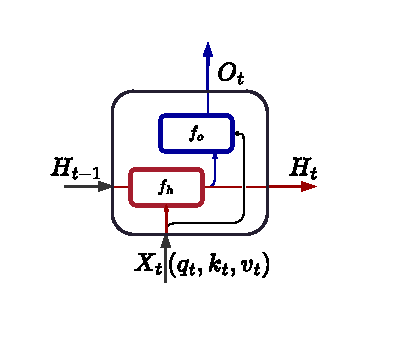
\includegraphics[width=0.9\linewidth]{images/part1/scheme-nonlinear.pdf}
    \caption{Единый вид моделей для обработки последовательностей с нелинейным обновлением состояния памяти.}
    \label{fig:scheme-nonlinear}
\end{figure}

\begin{align*}
&\textcolor{R}{H_t = f_h(H_{t-1}, x_t)} \\
&\textcolor{B}{o_t = f_o (H_t, x_t)} \\
\end{align*}

На временном шаге \( t \) состояние памяти обозначается как \( H_t \), а \( f_h \) представляет собой гейт записи в память, который контролируют её обновление, опираясь на текущий входной сигнал и предыдущее состояние памяти. В то же время \( f_o \) играет роль гейта чтения и формирования выхода, вычисляя значение \( o_t \) на текущем шаге. Этот подход напоминает концепцию, предложенную в~\cite{weston2014memory}, однако здесь операции обработки входа и обобщения сведены к одной операции. Для удобства также объединены выходная компонента и компонента отклика в единый механизм $f_o$.

\subsection{Единое представление моделей с линейным механизмом внимания}

Согласно~\cite{katharopoulos2020transformers, schlag2021linear}, линейные механизмы внимания формально соответствуют рекуррентным нейронным сетям (RNN), что позволяет относить их к моделям с пространством состояний.  

Рассмотрим механизм внимания, скалярном произведении:  

\[
o_i = V_i \text{ Softmax}(K_i^T q_i)
\]  

Если исключить операцию Softmax, это выражение можно преобразовать в рекуррентную форму, используя состояние памяти \( H_i \):  

\begin{align*}
& o_i = V_i (K_i^T q_i) = (V_i K_i^T) q_i = (\sum_{j=1}^i v_j k_j^T) q_i \\[1ex]
& \text{or}\\
& H_i = \sum_{j=1}^i v_j k_j^T \\
& \textcolor{R}{H_i = H_{i-1} + v_i k_i^T} \\
& \textcolor{B}{o_i = H_i q_i} \\
\end{align*}

Механизм линеаризованного внимания~\cite{katharopoulos2020transformers} можно представить в аналогичном виде:

\begin{align*}
& o_i = \sum_{j=1}^i \frac{v_j \kappa (k_j, q_i)}{\sum_{j'=1}^i \kappa (k_{j'}, q_i)} \\
& \text{replace } \kappa (k, q) = \phi(k)^T \phi(q) \\
& o_i = \sum_{j = 1}^i \frac{v_j \phi (k_j)^T \phi (q_i)}{\sum_{j'=1}^i  \phi (k_{j'})^T \phi(q_i)} \\
& \text{or}\\
% & H_i = \sum_{j=1}^i v_j k_j^T \\
& \textcolor{R}{H_i = H_{i-1} + v_i \phi(k_i^T)} \\
& \textcolor{B}{o_i = H_i \phi(q_i) / (z_t^T \phi(q_t))} \\
& \textcolor{B}{z_t = z_{t-1} + \phi(k_t)}
\end{align*}

По аналогии модели, в которых состояние памяти обновляется линейно, можно представить в следующем виде:
\begin{align*}
&\textcolor{R}{H_t = F_h (x_t) H_{t-1} + I_h(x_t)} \\
&\textcolor{B}{o_t = f_o (H_t, x_t)} \\
\end{align*}

\begin{figure}
    \centering
    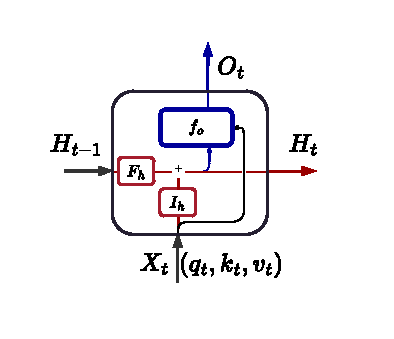
\includegraphics[width=0.9\linewidth]{images/part1/scheme-linear.pdf}
    \caption{Common view for sequence models with linear memory update.}
    \label{fig:scheme-linear}
\end{figure}

Операцию обновления \(f_h\) можно представить в линейной форме, разделив её на две составляющие: \(F_h\), отвечающую за забывание и сброс памяти, и \(I_h\), которая подготавливает входные данные перед их сохранением.

Этот подход, основанный на ключевых рекуррентных моделях, предложенных в~\cite{yang2024parallelizing}, позволяет описывать модели обработки последовательностей как с линейными обновлениями (Таблица~\ref{tab:overview-linear}), так и с нелинейными (Таблица~\ref{tab:overview-nonlinear}). Анализ операций с памятью способствует лучшему пониманию выразительности рассматриваемой архитектуры, а также её способности к поиску и использованию информации о последовательности.

Рассматривая линейные модели в Таблице~\ref{fig:scheme-linear}, можно выделить важность наличия операции забывания (Forget). Она необходим для сброса памяти, что особенно важно при работе с шумными данными или при смене контекста. Еще одним ключевым аспектом для обработки длинных и шумных последовательностей является возможность фильтрации входных данных перед их записью в память. Эту функцию выполняет операция обработки входа (Input) способность к фильтрации обеспечивается зависимостью данной операции от входной информации, как, например, в архитектуре Mamba. Практическая значимость этих функций подтверждается экспериментально в работе~\cite{gu2023mamba}. Стабильность обучения и масштаб представлений в памяти можно контролировать с помощью нормализующего скаляра \(z_t\), как это реализовано в нормализованных вариантах Linear Attention, mLSTM и ARMT. Эти аспекты должны учитываться учитывать при разработке новых линейных архитектур.

В нелинейных моделях размерность состояния памяти играет важную роль, так как она определяет емкость памяти. Операция записи в этих моделях объединяет обработку и фильтрацию входных данных, что делает важным её высокую выразительность и способность отсекать ненужную информацию. Операция чтения также должна быть эффективной, так как она напрямую влияет на скорость вывода. При этом она обязана обеспечивать достаточно высокое разрешение для доступа к большим контекстам или объемным кэшам памяти, если это предусмотрено архитектурой. Механизм внимания, часто комбинируемый с прямыми слоями и нормализацией слоев, остаётся доминирующим методом чтения из памяти. Однако, несмотря на его эффективность, масштабируемость таких подходов обходится дорого с вычислительной точки зрения, а качество может снижаться при увеличении размера памяти. Это подчеркивает актуальность использования механизмов выборки или фиксированных размеров памяти в ряде случаев.


\begin{table*}[t!]

\footnotesize
\scalebox{0.87}{
\begin{tabular}{l llll}
\toprule
   Model  & Forget $F_h$ & Input $I_h$ & Read $f_o$ & Normalization $z_t$ \\
   \midrule
   Linear RNN &  $W_{hh}$  &  $x_t W_{xh} + b_h$  &  $\phi (H_t W_{ho} + b_o)$  &  1 \\
    Linear Attention \cite{katharopoulos2020transformers} &  1  &  $v_t k_t^T$  & $H_t q_t$  &  1  \\
        \,\, + Kernel &  1  &  $v_t \phi(k_t)^T$  & $H_t \phi(q_t)$  &  1  \\
\,\, + Normalization &  1  &  $v_t \phi(k_t)^T$  & $H_t \phi(q_t) / (z_t^T \phi (q_t))$  &  $z_{t-1} + \phi(k_t)$  \\
    DeltaNet~\cite{schlag2021linear} & $I - \beta_t k_t k_t^T$  &  $\beta_t v_t k_t^T$  &  $H_t q_t$  &  1  \\
    RetNet \cite{sun2023retentive} &  $\gamma$  &  $v_t k_t^T$  & $H_t q_t$  &  1  \\
    RWKV-6 \cite{peng2023rwkv} &  $\text{Diag}(\alpha_t)$  &  $v_t k_t^T$  & $(H_{t-1} + (d \odot v_t) k_t^T) q_t$  &  1  \\
    S4 \cite{gu2021s4} &  $\text{exp}(-\alpha 1^T) \odot \text{exp}(A)$  &  $B \odot (v_t 1^T)$  & $(H_t \odot C) 1 + d \odot v_t $ &  1  \\
    Mamba \cite{gu2023mamba} &  $\text{exp}(-\alpha_t 1^T) \odot \text{exp}(A)$  &  $(\alpha_t \odot v_t) k_t^T$  & $H_t q_t + d \odot v_t$  &  1  \\
    Mamba-2 \cite{dao2024transformers} &  $\gamma_t$  &  $v_t k_t^T$  & $H_t q_t$  &  1  \\
    mLSTM  \cite{beck2024xlstm} &  $f_t$  &  $i_t v_t k_t^T$  & $H_t q_t / \max \{ 1, |z_t^T q_t | \}$ &  $f_t z_{t-1} + i_t k_t$  \\
    \midrule
    ARMT  \cite{rodkin2024associative} &  1  &  $\beta_i (v_i - \overline{v_i}) \otimes \phi(k_i)$  & $H_t \phi (q_j) / (z_t^T \phi (q_j))$  &  $z_{t-1} + \gamma \phi (k_i)$  \\
    \bottomrule
\end{tabular}}

\vspace{1mm}
\caption{Операции с памятью в моделях с линейным обновлением памяти изображены на рисунке~\ref{fig:scheme-linear}. Запись осуществляется с помощью линейного преобразования, которое состоит из двух основных компонентов: гейта забывания Forget, регулирующего поток данных от предыдущего временного шага, и гейта входа Input, который вносит информацию из входных данных модели в состояние памяти \( H_t \). Для сохранения стабильности масштаба используется нормировочная константа \( z_t \).}
\label{tab:overview-linear}
\end{table*}


\begin{table*}[t!]

\footnotesize
\scalebox{0.87}{
\begin{tabular}{l lll}
\toprule
   Model  & Memory $H_t$ & Write $f_h$ & Read $f_o$ \\
   \midrule
   RNN  &  $h_t$  &  $h_t = \phi( h_{t-1} W_{hh} + x_t W_{xh} + b_h)$  &  $\phi(h_t W_{ho} + x_t W_{xo} + b_o)$  \\
   LSTM~\cite{lstm1999hochreiter}  &  $(h_t, o_t)$  &  $h_t = f_t \odot h_{t-1} + i_t \odot \tilde{h}_t$  &  $o_t = \tilde{o}_t \odot \text{tanh}(h_t)$ \\
   Attention~\cite{bahdanau2015neural} & \begin{tabular}{@{}l@{}}$H^e = \{h_{\tau}^e\}_{\tau = 1}^T$ \\ $h_t^{d (1 \times d)}$ \end{tabular} & \begin{tabular}{@{}l@{}}$c_t = \sum_{\tau = 1}^t \alpha(s_{t-1}, h_{\tau}^e) h_{\tau}^e$ \\ $h_t = f(h_{t-1}, y_{t-1}, c_t)$ \end{tabular}  &  $g(y_{i-1}, h_i, c_i)$  \\
   Memory Networks~\cite{weston2014memory}  &  $H^{m \times d}$  & $H_t[i] = G(H_{t-1}[i], I(x_t), H_{t-1})$  &  $(R \circ O)(I(x_t, m_t) $ \\
   NTM~\cite{graves2014neural}  &  $H^{m \times d}$ &  \begin{tabular}{@{}l@{}} $\tilde{H}_t[i] = H_{t-1}[i] (1 - w_t[i] e_t)$ \\ $H_t[i] = \tilde{H}_t[i] + w_t a_t$ \end{tabular} &  $\sum_{i=1}^m w_t[i] H_t[i]$  \\
   \midrule
   Transformer~\cite{vaswani2017attention} & \begin{tabular}{@{}l@{}} $H^{e} = \{h_{\tau}^e\}_{\tau = 1}^T$ \\ $H_t = \{h_{\tau}\}_{\tau = 1}^t$ \end{tabular}   &  \begin{tabular}{@{}l@{}}$c_t = \text{MHA}_{\text{self}}(h_t, H_t)$ \\ $\tilde{h}_t = \text{MHA}_{\text{cross}}(c_t, H^e)$ \end{tabular}  & $\tilde{\text{FF}} (\tilde{h}_t)$ \\
   \midrule
   Transformer-XL~\cite{dai2019transformerxl} & $H_t^c = \{h_{\tau}^c\}_{\tau = \text{max}\{\tau_0 -c, 0\}}^{\tau_0}$  &  $h_{\tau}^c = h_{\tau}, \tau \in [\text{max} \{ \tau_0 - c, 0 \}, \tau_0]$  &  $\text{TrLayer}(h_t, [H_t^c, H_t])$ \\
   MT~\cite{burtsev2020memory-transformer} & $H^m = \{h_i\}_{i = 1}^{m}$  &  $\tilde{h}_i^m = \text{TrLayer}^m(h_i^m, [H^m, H_t])$ & $\text{TrLayer}(h_t, [H^m, H_t])$ \\
   RMT~\cite{bulatov2022recurrent} &  $H^m = \{h_i\}_{i = 1}^{m}$  &  $\tilde{h}_i^m = \text{TrLayer}(h_i^m, [H^m, H_t])$ & $\text{TrLayer}(h_t, [H^m, H_t])$ \\
   \midrule
   Retrieval-augmented generation &  $H^c = \{h_i^c\}_{i=1}^m$  &  $h_i^c = \text{TrLayer}^e(h_i, H_t)$ & $\text{TrLayer}(h_i, [\text{kNN}(H^m, H_t), H_t])$ \\
    \bottomrule
\end{tabular}}


\vspace{1mm}
\caption{Операции памяти для моделей с нелинейным обновлением памяти (Рисунок~\ref{fig:scheme-nonlinear}). В данном случае $H_t$ обозначает состояние памяти, а функции $f_h$ и $f_o$ соответствуют операциям записи и чтения.}  
\label{tab:overview-nonlinear}  
\end{table*}  


\section{Различия в представительных возможностях с точки зрения работы с памятью}  
\label{sec:differences}  

Рекуррентные нейронные сети (RNN) и трансформеры представляют два противоположных подхода к организации памяти. RNN работают с компактной памятью фиксированного размера, которая обновляется на каждом временном шаге. В отличие от них, трансформеры используют несжатую память, хранящую информацию обо всех временных шагах и обеспечивающую одновременный доступ ко всем данным. Эти различия формируют различные требования к вычислительным ресурсам и памяти, а также влияют на задачи, которые каждая из архитектур способна решать.  

\textbf{Вычислительная эффективность.}
В любой момент времени RNN работают только с одним состоянием памяти, что обеспечивает постоянный объём памяти, не зависящий от размера контекста. Также сложность каждой операции обращения к памяти составляет $O(1)$, что делает RNN удобными для применения в условиях ограниченных ресурсов. С другой стороны, трансформеры используют кэш ключей и значений, который линейно увеличивается с размером контекста, требуя $O(N)$ памяти. Кроме того, вычислительные затраты на чтение из памяти возрастают квадратично из-за использования механизма внимания.  

\textbf{Эффективность обучения.}
Благодаря высокой степени параллелизма трансформеры легко и эффективно обучаются на современных вычислительных устройствах. В отличие от них, обучение RNN представляет сложности из-за отсутствия параллельных вычислений и проблем с распространением градиентов через большое число временных шагов. Чтобы решить эти проблемы, современные RNN применяют подходы, такие как свёрточные представления и линейное обновление памяти~\cite{gu2020hippo, gu2021s4, gu2023mamba, peng2023rwkv}, которые улучшают параллелизацию во время обучения.  

\textbf{Компромисс между сжатием и пропускной способностью}~\cite{arora2024simple}.  
Для RNN характерно сжатие всей информации о прошлом в фиксированное состояние памяти, что зачастую приводит к потере данных. Кроме того, взаимодействие представлений временных шагов, разделённых интервалом $\Delta t$, возможно только после выполнения $O(\Delta t)$ операций, что усложняет задачи, такие как разрешение кореференций. Трансформеры же сохраняют несжатые представления всех временных шагов, обеспечивая богатый контекст и минимальные потери, поскольку все элементы памяти взаимодействуют на каждом слое.  

\textbf{Глубина представлений.}
RNN непрерывно обновляют память на каждом временном шаге, что создаёт более глубокие представления. За $N$ временных шагов память обновляется $O(N)$ раз, что позволяет эффективно работать с длинными контекстами. В трансформерах глубина представлений фиксирована числом слоёв. Однако их структура позволяет токенам взаимодействовать друг с другом параллельно, делегируя часть задач соседним токенам.  

\textbf{Разрешающая способность.}
Высокая гранулярность представлений памяти Трансформеров могут вызывать трудности при обработке большого объёма нерелевантной информации, как, например, в задачах с длинными контекстами, что приводит к явлению «пересжатия» данных~\cite{barbero2024transformers}. Исследования~\cite{liu2023lost, hsieh2024ruler, kuratov2024babilong} указывают на значительное снижение качества поиска информации в таких случаях, связанное с шумом, вызванным избыточной детализации представлений. С другой стороны, унифицированная, но ограниченная по объёму память RNN также создаёт проблемы при увеличении длины контекста~\cite{jelassi2024repeat}.  


\section{Потенциальная выразительность нейронных архитектур}

Современные исследования показывают высокую выразительную способность как трансформеров, так и современных RNN. Однако важно понимать, в каких условиях каждая из архитектур наиболее эффективна.  

Одним из ключевых преимуществ трансформеров является их способность извлекать конкретные элементы из предыдущего ввода. Например, ~\cite{jelassi2024repeat} демонстрирует, что трансформеры с определёнными позиционными кодировками превосходят обобщённые модели пространств состояний (GSSM) в задачах копирования до тех пор, пока состояние памяти GSSM не масштабируется линейно с длиной последовательности. Это преимущество распространяется и на реальные задачи, требующие извлечения данных~\cite{park2024can, waleffe2024empirical}.  

И RNN, и механизмы внимания теоретически являются Тьюринг-полными при наличии неограниченного числа промежуточных вычислительных шагов~\cite{chen2017recurrent, perez2019turing, perez2021attention, siegelmann1994analog}. Дальнейшие исследования~\cite{deletang2022neural, strobl2024formal} показывают их практическую значимость, учитывая такие факторы, как точность и глубина вычислений.  

Формальные языки предоставляют полезный инструмент для оценки выразительности этих архитектур. В частности, выразительная способность RNN долгое время анализировалась через задачи, связанные с иерархией Хомского~\cite{gers2001lstm, deletang2022neural}, а современные исследования~\cite{strobl2024formal} выявляют различия в том, как трансформеры и RNN справляются с определёнными формальными языками. Например, RNN способны представлять все регулярные языки~\cite{korsky2019computational} и, используя дополнительные подходы, такие как рассуждения по цепочке~\cite{merrill2023expresssive}, расширять свою выразительность. Расширение памяти является ключевым подходом для повышения этих возможностей~\cite{das1992learning, suzgun2019memory, deletang2022neural}, предоставляя инструменты для улучшения обобщающей способности и адаптации к различным задачам.  

\section{Классификация нейронных архитектур с расширенной памятью}
\label{sec:taxonomy}  

В данном разделе представлена классификация нейронных моделей, основанная на характеристиках их механизмов памяти. Определяются ключевые свойства памяти и анализируется их влияние на экспрессивность моделей. В случае использования несколькими типами памяти акцент делается на основном механизме (например, XL-кэш для Transformer-XL).  

\textit{Назначение (Dimension)}. Память может использоваться для сохранения информации во времени (\textit{Length}), хранения промежуточных вычислений (\textit{Depth}) или обоих аспектов (\textit{d + l}). Память во времени улучшает моделирование долгосрочных зависимостей, а память, ориентированная на глубину, поддерживает сложные вычисления, требующие длительного хранения данных.  

\textit{Context (Размер контекста)} варьируется в зависимости от механизма памяти. Для моделей на основе внимания она может быть ограничена, например, объёмом vRAM, тогда как для RNN теоретически возможен неограниченный контекст.  

Функции \textit{Чтение (Read)} и \textit{Запись (Write)} определяют выразительность памяти. Адресация может выполняться по \textit{локации (Location)}, \textit{контексту (Context)} или обоим параметрам. Возможности \textit{фильтрации (Filtering)} и \textit{забывания (Forgetting)} дополнительно улучшают управление памятью, повышая устойчивость к шуму и результаты на задачах, связанных с длительным хранением данных~\cite{gu2023mamba}.  

Другая характеристика памяти - \textit{срок жизни (Lifetime)} Некоторые виды памяти, такие как ассоциативные или медленные веса, остаются неизменными на всем протяжении использования модели, тогда как в других моделях, например RNN, состояния памяти сбрасываются после обработки каждой последовательности.

\textit{Размер хранилища (Storage size)} и \textit{число слоев (Layers)} влияют на глубину и объём памяти. Хотя оценка практической ёмкости памяти является сложной задачей, размерность памяти служит базовым ориентиром.  


\begin{table*}[ht]
\centering
\tiny
\caption{Таксономия механизмов памяти в нейросетевых архитектурах}
\label{tab:taxonomy}
\begin{tabular}{lllllllllll}
\toprule
           Model & Dimension &  Lifetime &   Layers &      Context &   Addressing &             Read &                  Write &         Filtering &     Forgetting &             Storage size \\
\midrule
    Fast Weights &    length &    sample &        1 &     infinite &      content &               ff &          outer product &                 - &              - &                $state^2$ \\
Hopfield Network &    length & unlimited &        1 &      1 query &      content &      update rule &          outer product &                 - &              - &                $state^2$ \\
 Hopfield Layers &    length & unlimited & n layers &       window &      content &      update rule &              attention &                 - &              - &                $state^2$ \\
             RNN &    length &    sample &        1 &     infinite &      content &               ff &                     ff &                 - &              - &                    state \\
            LSTM &    length &    sample &        1 &     infinite &      content &       input gate &                     ff &        input node &    forget gate &                  state*2 \\
              S4 &     l + d &    sample &        1 &     infinite &      content &               ff &                     ff &                 - &              - &                    state \\
            RWKV &     l + d &    sample &        1 &     infinite &          NaN &               ff &                     ff &                 - &              - &                    state \\
           Mamba &     l + d &    sample &        1 &     infinite &      content &               ff &           ff+selection &         selection &      selection &                    state \\
       Attention &    length &    sample &        1 &     infinite &      content &        attention &                     ff &                 - &              - &                      NaN \\
          MemNet &    length &    sample &        1 &     infinite & c + location &        attention &              attention &    generalization & generalization &                      NaN \\
      E2E MemNet &    length &    sample &        1 &     infinite &        c + l &        attention &              attention &    generalization & generalization &                      NaN \\
             NTM &    length &    sample &        1 &     infinite &        c + l &        attention &            erase + add &        add vector &     erase gate & state size * memory size \\
     Transformer &    length &    sample & n layers &       window &        c + l &        attention &              attention &   skip connection &              - &             window*state \\
   Universal Tr. &    depth  &    sample & n layers &       window &        c + l &        attention &              attention &   skip connection &              - &             window*state \\
      Memory Tr. &     depth &    sample &        1 &       window &        c + l &        attention &              attention &   skip connection &              - &             state*memory \\
      Longformer &     l / d &    sample &        1 &       window &        c + l &        attention &              attention &   skip connection &              - &             state*memory \\
          Tr.-XL &    length &    sample & n layers & W * n layers &        c + l &        attention &              attention &                 - &              - &    (cache+window)*state  \\
             RMT &     l + d &    sample &        1 &     infinite &        c + l &        attention &              attention &   skip connection &              - &             state*memory \\
            ARMT &    length &    sample & n layers &     infinite &        c + l & linear attention & attention + delta rule & importance scalar &     delta rule &           layers*d qk\^2 \\
          MemGPT &     l + d & unlimited &        1 &     infinite &      content &        attention &              attention &   skip connection &              - &                    cache \\
  AutoCompressor &     l + d &    sample &        1 &   W *  n seg &        c + l &        attention &              attention &   skip connection &              - &       state*memory*n seg \\
  Memorizing Tr. &    length & unlimited &        1 &    W + cache &      content &    knn+attention &                   none &                 - &              - &                    cache \\
           RETRO &    length & unlimited & n layers &    W + cache &      content &    knn+attention &                   none &                 - &              - &                    cache \\
             RPT &    length &    sample &        1 &    W + cache &      content &    knn+attention &                   none &                 - &              - &                    cache \\
    Unlimiformer &    length & unlimited & n layers &    W + cache &      content &    knn+attention &                   none &                 - &              - &                    cache \\
\bottomrule
\end{tabular}

\end{table*}


\subsection{Transformer с дополнительной памятью}

Transformer сталкивается с рядом ограничений, особенно при обработке длинных контекстов и сложных задач. В данном разделе рассматриваются решения, основанные на памяти, для преодоления этих ограничений, повышения эффективности обработки и улучшения архитектуры.  

В Transformer память хранится в скрытых состояниях, которые передаются через механизм внимания. Однако те же скрытые состояния и веса модели используются как для операций с памятью, так и для выполнения основной задачи, такой как предсказание следующего токена. Это приводит к смешению локальных и глобальных признаков в одном и том же представлении, что ограничивает ёмкость и гибкость модели. Memory Transformer (MT)~\cite{burtsev2020memory-transformer} решает эту проблему, вводя глобальные токены в качестве выделенного хранилища для глобального контекста и промежуточных результатов. Эти токены памяти обрабатываются вместе с входными данными, причём некоторые варианты MT используют отдельные веса для операций с памятью.  

\begin{align*}
& \textcolor{B}{h_t^L = FF(s_t^L) } \\
& \textcolor{B}{s_t^{L} = MHA(c_t^L, \tilde{H}^L_{t} ) } \\
& \textcolor{B}{\tilde{H}^L_{t} = [M^{L-1} \circ H_{t}^{L-1}]} \\[1ex]
& \textcolor{R}{M^{L} = [m_{1}^L, ..., m_{mem}^L]} \\[1ex]
& \textcolor{R}{m_{i}^{L} = FF(MHA(m_{i}^L, \tilde{H}^L_{t}))} \\[1ex]
\end{align*}


Память в Memory Transformers (MT) имеет отличное от ранее рассмотренных подходов назначение и больше связана с концепцией рабочей памяти. Схожая архитектура используется в методах prompt- и prefix-tuning~\cite{lester2021power, li2021prefix}, где оптимизируются префиксы для входных данных слоёв Transformer, при этом основные параметры модели остаются неизменными. Это позволяет модели включать специфические для задачи знания без изменения её основных весов. Однако, несмотря на архитектурное сходство, MT обладает большей потенциальной выразительностью, так как её тренируемые веса могут изучать новые операции, используя добавленную память.  

Добавление дополнительных токенов также решает ключевую проблему Transformers. Парные взаимодействия между состояниями памяти приводят к квадратичной вычислительной сложности относительно размера входных данных, что делает расширение окна внимания и захват долгосрочных зависимостей всё более затратными. Со временем было предложено множество методов для смягчения этой проблемы. Один из подходов заключается в разрежении маски внимания при минимизации потерь покрытия входных данных. Например, Longformer~\cite{beltagy2020longformer} ограничивает расстояние внимания заранее заданным диапазоном, используя механизм скользящего окна. Чтобы обеспечить взаимодействие между более удалёнными токенами, вводятся глобальные токены, которые могут обращаться ко всем токенам в последовательности и быть доступными для всех токенов на разных слоях. Big Bird~\cite{zaheer2020big} расширяет покрытие входных данных, добавляя случайное разреженное внимание, что позволяет сохранить линейную сложность при поддержании эффективности. Глобальные токены также помогают стабилизировать генерацию длинных текстов в моделях со скользящим окном~\cite{xiao2023efficient}.  

Хотя добавление глобальных токенов влечёт за собой небольшие вычислительные затраты по сравнению с базовой моделью, эти затраты зачастую незначительны в контексте общей стоимости модели. Усиление архитектур за счёт глобальных токенов обычно приводит к улучшению результатов в сложных задачах. Однако при обработке длинных контекстов модели с разреженным вниманием и глобальной памятью всё ещё уступают по эффективности более дорогим моделям с полным вниманием, которые обеспечивают лучшие результаты. Глобальные токены также играют важную роль в экономически эффективных методах обучения, таких как prompt-tuning и prefix-tuning.  
.

\section{Трансформеры с дополнительным механизмом извлечения информации}
\label{sec:retrieval}

Сжатие представлений в фиксированное пространство памяти связано с риском потери информации. Альтернативный подход состоит в хранении всех обработанных данных в расширяемом несжатом хранилище. Однако, по мере роста объема хранилища, операции внимания становятся вычислительно затратными. Для сокращения этих затрат часто применяют метод поиска ближайших соседей ($k$NN), который широко используется в задачах информационного поиска.

Например, Memorizing Transformer~\cite{wu2022memorizing} сохраняет все скрытые состояния из определенного слоя трансформера и извлекает релевантные данные для текущего контекста с помощью метода $k$NN. Эти данные используются как ключи и значения для механизмов внимания, а результаты их обработки комбинируются через обучаемый шлюз для выполнения поставленной задачи. Unlimiformer~\cite{bertsch2023unlimiformer} расширяет подобный механизм извлечения на все слои и головы предобученных трансформеров, применяя уже существующие параметры модели без добавления новых. Retro~\cite{borgeaud2022retro} масштабирует подходы извлечения до крупных моделей (до 7,5 миллиардов параметров) и огромных баз данных, содержащих до триллионов токенов, для оценки языковых моделей и задач на downstream. Retrieval-Pretrained Transformer~\cite{rubin2023long} обучается с нуля для выполнения задач самопоиска, извлекая семантически близкие сегменты из ранее обработанного контекста для улучшения предсказания токенов. Также вводится дополнительная функция потерь для предсказания следующего сегмента, что улучшает точность извлечения.

Использование дополнений через поиск позволяет значительно расширить область действия внимания без необходимости квадратичного увеличения вычислительных затрат. Это достигается за счет хранения большого объема несжатой памяти в расширяемом хранилище с упрощенными операциями чтения. Однако такая простота операций имеет свои ограничения: семантический поиск часто игнорирует временную структуру данных, что снижает его эффективность в задачах, требующих многошагового рассуждения или более сложных методов извлечения~\cite{li2024retrieval, kuratov2024babilong}. Одним из способов решить данные ограничения является Трансформеры с рекуррентностью на уровне сегментов, данные модели рассмотрены в следующей Главе~\ref{ch:ch2}.

\section{Связанные обзорные работы}

Концепция памяти оказала значительное влияние на формирование многих классических основ, которые легли в основу современных архитектур. Работы ~\cite{rumelhart1986parallel, mcclelland1987parallel} описали принципы параллельной распределенной обработки, открыв возможность создания систем, способных к сложному принятию решений. Такие системы включают функции, аналогичные когнитивным способностям человека, например, восприятие и память. ~\cite{elman1990finding} акцентировал внимание на особенностях задач с временными зависимостями и предложил нейронные архитектуры, такие как рекуррентные сети, популярность и применение которых значительно возросли благодаря этому исследованию.

Работа ~\cite{tay2020efficient} представляет систематический анализ модификаций трансформеров с точки зрения эффективности, уделяя внимание обработке длинных контекстов, оптимизации вычислений и улучшению работы с памятью. ~\cite{cherepanov2024unraveling} разрабатывают классификацию типов памяти, актуальных для агентов обучения с подкреплением. Исследование ~\cite{he2024human} сосредоточено на аналогиях между механизмами задач машинного обучения, использующих память, и типами долговременной памяти человека. Обзор~\cite{khosla2023survey} также рассматривает ключевые архитектуры, дополненные памятью, но в контексте процессов, происходящих в мозге.

% \section{Заключение}

% В данной статье проведён обзор ключевых нейронных архитектур через призму концепции памяти. Рассматриваются модели, использующие медленное и быстрое хранение, механизмы ассоциативной памяти, а также подходы к обработке последовательностей.

% Мы разработали концептуальную основу для унифицированного представления линейных и нелинейных архитектур обработки последовательностей. Используя эту основу и результаты других исследований, мы изучили сходства и различия между параллельными и последовательными моделями. В частности, мы детализировали структурные и функциональные сходства между моделями линейного внимания и рекуррентными нейронными сетями, а также уточнили их различия с математической точки зрения. Дополнительно предложена память-ориентированная интерпретация для нелинейных моделей и обозначены перспективные направления их развития. Мы уверены, что наш подход будет полезен для дальнейших исследований нейронных архитектур с дополнением памяти и моделей, предназначенных для работы с последовательностями.